% Asal-usul (tidak pernah dicetak): lihat sources/outline_sources.md (Tahun 1: struktur vertikal atmosfer, laju lapse, suhu potensial dan stabilitas statis; samudra berlapis, persamaan keadaan air laut, diagram T-S dan massa air). Nilai soal latihan dan soal dalam kalkulator skrap Buku 3 calc/ch26.py; gambar dari figdata/bachelor-1/atmosphere_profile.py (Atmosfer Standar AS 1976) dan seawater_eos.py (EOS-80 dan algoritma UNESCO 44; kolom WOA23, dataset bachelor-1-woa23-* dan grade-10-woa23-arctic-* Buku 2). Fisika memiliki hubungan hidrostatik, atmosfer isotermal dan tinggi skalanya, hukum pertama, relasi Laplace, dan daya apung Archimedes (diingat kembali). Buku 1 (kelas 8) memberi lapisan-lapisan dan laju lapse lingkungan 6,5 K/km; Buku 2 (kelas 10) laju adiabatik kering yang diterima, udara stabil dan tidak stabil, lapisan campuran, termoklin, haloklin dan piknoklin: didirikan ulang di sini dengan penurunan. Adiabat lembap milik volume Tahun ke-2.
\chapter{Struktur atmosfer dan samudra}\label{ch:b1:fluid-envelopes-structure}

Dua kali sehari, di stasiun cuaca di seluruh dunia, sebuah balon dilepaskan membawa sebuah radiosonde, instrumen kecil yang mengirimkan kembali lewat radio tekanan, suhu dan kelembapan udara saat ia naik; ia naik sekitar \qty{300}{m} per menit dan dapat mencapai \qty{35}{km} sebelum balonnya pecah. Jauh di laut, sebuah kapal riset menurunkan bingkai instrumen dan botol-botol air dengan kabel ke jurang, mengukur konduktivitas, suhu dan kedalaman sepanjang perjalanan. Kedua profil itu, satu dari udara dan satu dari air, adalah bahan mentah bab ini. Kedua selubung itu berlapis, dan di keduanya pelapisan ditentukan oleh massa jenis: fluida ringan di atas fluida berat. Apa yang membuat suatu lapisan ringan atau berat kurang jelas daripada kelihatannya. Udara yang lebih dingin daripada udara di bawahnya tetap bisa lebih ringan; air yang lebih hangat daripada air di atasnya tetap bisa lebih berat. Bab ini membangun dua alat untuk memilah hal ini, \omterm{def:b1:fluid-envelopes-structure:potential-temperature}{suhu potensial} dan \omterm{def:b1:fluid-envelopes-structure:eos}{persamaan keadaan air laut}.
% ledger: nws:radiosonde, nws:radiosonde-def, commons:ctd-rosette

\begin{omfigure}
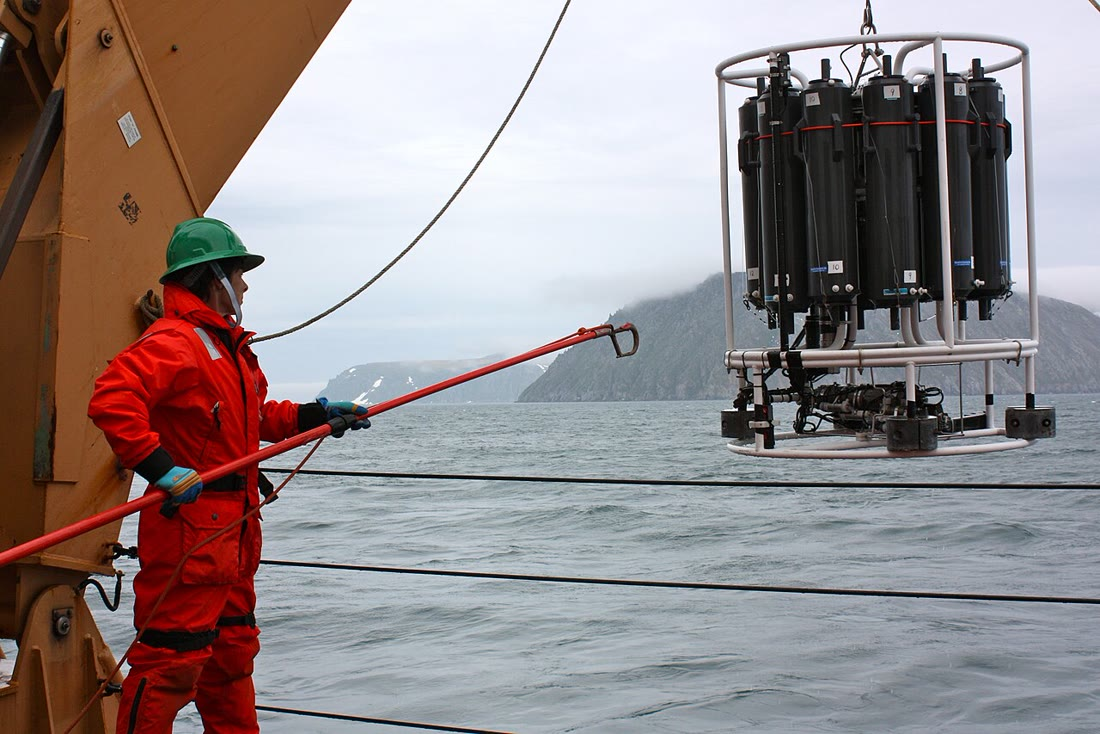
\includegraphics[width=0.62\linewidth]{images/book3/b1-ctd-rosette.jpg}

{\small CTD dan rosette dibawa ke atas kapal di Selat Bering pada Juni 2011. Botol-botol abu-abu di sekeliling bingkai ditutup pada kedalaman yang dipilih dalam perjalanan ke atas untuk mengambil sampel air; instrumen di bagian bawah bingkai mengukur konduktivitas (dari situ salinitas dihitung), suhu dan kedalaman (sebenarnya tekanan) secara terus-menerus saat bingkai diturunkan. (NASA Pusat Penerbangan Antariksa Goddard, domain publik, melalui Wikimedia Commons.)}
\label{fig:b1:fluid-envelopes-structure:ctd}
\end{omfigure}
% ledger: commons:ctd-rosette, unesco44:atg-theta

\begin{recall}
Buku-buku fisika memberikan hubungan hidrostatik, $\mathrm dp/\mathrm dz =
-\rho g$, untuk fluida diam; untuk gas ideal dengan massa molar $M$, $p = \rho R
T/M$, dan dalam atmosfer isotermal tekanan turun sebagai $e^{-z/H}$ dengan tinggi
skala $H = RT/(Mg)$. Mereka menyatakan hukum pertama untuk sistem tertutup dan,
untuk gas ideal, relasi Laplace sepanjang transformasi adiabatik reversibel,
$pV^{\gamma} = $ konstan, dengan $\gamma = c_p/c_v$ dan $c_p - c_v
= R/M$ per satuan massa. Benda yang tercelup dalam fluida menerima daya apung ke
atas yang sama dengan berat fluida yang dipindahkannya (Archimedes). Buku~1 menamai
lapisan atmosfer dan \omterm{def:b1:fluid-envelopes-structure:lapse-rate}{laju lapse lingkungan} \omterm{def:b1:fluid-envelopes-structure:standard-atmosphere}{atmosfer standar}, \qty{6.5}{\celsius} per
kilometer di troposfer; Buku~2 menerima \omterm{def:b1:fluid-envelopes-structure:lapse-rate}{laju adiabatik kering}, \qty{9.8}{\celsius}
per kilometer, menyebut udara stabil atau tidak stabil menurut nasib sebuah parsel
yang didorong ke atas, dan menjelaskan \omterm{def:b1:fluid-envelopes-structure:ocean-layers}{lapisan campuran}, \omterm{def:b1:fluid-envelopes-structure:ocean-layers}{termoklin}, \omterm{def:b1:fluid-envelopes-structure:ocean-layers}{haloklin} dan
\omterm{def:b1:fluid-envelopes-structure:ocean-layers}{piknoklin} samudra. Salinitas air laut mendekati 35 gram garam terlarut per kilogram.
% ledger: ussa76:layers, nws:dalr, nos:salinity
\end{recall}

\section{Struktur vertikal atmosfer}\label{sec:b1:fluid-envelopes-structure:atmosphere}

Tidak ada profil nyata yang sama dengan profil berikutnya. Untuk membandingkannya, sebuah profil acuan ditetapkan dengan konvensi.

\begin{definition}[Atmosfer standar]\label{def:b1:fluid-envelopes-structure:standard-atmosphere}
Sebuah \emph{atmosfer standar}\index{atmosfer standar} adalah profil suhu, tekanan dan massa jenis terhadap ketinggian yang ditetapkan dengan konvensi: udara kering dengan massa molar konstan, gas ideal dalam keseimbangan hidrostatik, dengan nilai tertentu di permukaan laut dan suhu yang bervariasi linear terhadap ketinggian dalam lapisan-lapisan berurutan. Atmosfer standar 1976 mengambil \qty{288.15}{K} dan \qty{101325}{Pa} di permukaan laut, $M_0 = \qty{28.9644}{kg.kmol^{-1}}$, $R^* = \qty{8314.32}{J.kmol^{-1}.K^{-1}}$ dan $g_0 = \qty{9.80665}{m.s^{-2}}$.
\end{definition}
% ledger: ussa76:sea-level

Di bawah \qty{47}{km} \omterm{def:b1:fluid-envelopes-structure:standard-atmosphere}{atmosfer standar} 1976 memiliki empat lapisan (\cref{tab:b1:fluid-envelopes-structure:layers}). Yang terendah, troposfer, mendingin sebesar \qty{6.5}{K} per kilometer; dari puncaknya, tropopause, suhu tetap \qty{216.65}{K} selama sembilan kilometer, lalu naik. Ketinggian standar adalah ketinggian geopotensial, ketinggian yang akan diberikan oleh gravitasi konstan $g_0$ dengan energi potensial yang sama; di bawah \qty{32}{km} mereka berbeda dari ketinggian geometris kurang dari \qty{0.6}{\percent} (\qty{11}{km} dari standar terletak di \qty{11.02}{km}).
% ledger: ussa76:layers, ussa76:sea-level

\begin{table}[ht]
\centering
\small
\renewcommand{\arraystretch}{1.2}
\begin{tabular}{|l|c|c|c|c|}
\hline
Lapisan & Dasar (km) & $\mathrm dT/\mathrm dz$ (K/km) & $T$ di dasar (K) & $p$ di dasar (hPa) \\
\hline
1 (troposfer) & 0 & $-6.5$ & 288.15 & 1013.25 \\
2 (stratosfer) & 11 & 0.0 & 216.65 & 226.32 \\
3 (stratosfer) & 20 & $+1.0$ & 216.65 & 54.75 \\
4 (stratosfer) & 32 & $+2.8$ & 228.65 & 8.68 \\
\hline
\end{tabular}
\caption{Empat lapisan terendah \omterm{def:b1:fluid-envelopes-structure:standard-atmosphere}{atmosfer standar} 1976. Gradien dan nilai permukaan laut adalah nilai pendefinisian; suhu dan tekanan di dasar dihitung darinya dengan \cref{prop:b1:fluid-envelopes-structure:layer-pressure}.}
\label{tab:b1:fluid-envelopes-structure:layers}
\end{table}
% ledger: ussa76:layers, ussa76:sea-level (bases computed in figdata/bachelor-1/atmosphere_profile.py)

Dalam setiap lapisan suhu adalah fungsi linear dari ketinggian, sehingga relasi hidrostatik dapat diintegrasikan dalam bentuk tertutup.

\begin{proposition}[Tekanan dalam lapisan gradien konstan]\label{prop:b1:fluid-envelopes-structure:layer-pressure}
Dalam lapisan udara kering di mana $T = T_b - L\,(z - z_b)$ dengan $L \neq 0$ konstan, tekanannya adalah
\[
  p = p_b \left(\frac{T}{T_b}\right)^{gM/(RL)},
\]
dengan $T_b$ dan $p_b$ adalah nilai di dasar $z_b$. Ketika $L = 0$ tekanan turun secara eksponensial dengan tinggi skala $H = RT_b/(Mg)$.
\end{proposition}

\begin{proof}
Relasi hidrostatik dan gas ideal memberikan $\mathrm dp/p = -(gM/R)\,\mathrm
dz/T$. Karena $\mathrm dT = -L\,\mathrm dz$, ini adalah $\mathrm dp/p =
(gM/(RL))\,\mathrm dT/T$, yang diintegrasikan menjadi $\ln(p/p_b) = (gM/(RL))
\ln(T/T_b)$. Untuk $L = 0$, $T = T_b$ dan $\ln(p/p_b) = -(z - z_b)/H$: atmosfer isotermal dari volume fisika.
\end{proof}

Di troposfer standar, $gM/(RL) = 9.80665 \times 28.9644 /
(8314.32 \times 0.0065) = 5.256$, dan pada \qty{11}{km}, $T = 216.65$~K:
$p = \num{101325} \times (216.65/288.15)^{5.256} = \qty{22632}{Pa}$, sedikit di bawah seperempat nilai permukaan laut. Dalam lapisan isotermal di atasnya, $H =
8314.32 \times 216.65/(28.9644 \times 9.80665) = \qty{6.34}{km}$, dan sembilan kilometer lebih tinggi tekanan telah turun dengan faktor tambahan $e^{9/6.34} =
4.13$, menjadi \qty{5475}{Pa}. Karena tekanan pada suatu level adalah berat, per satuan luas, udara di atasnya, setengah massa \omterm{def:b1:fluid-envelopes-structure:standard-atmosphere}{atmosfer standar} terletak di bawah \qty{5.5}{km} dan sembilan persepuluh di bawah \qty{16}{km}.
% ledger: ussa76:sea-level, ussa76:layers (values computed in figdata/bachelor-1/atmosphere_profile.py)

\section{Laju lapse dan suhu potensial}\label{sec:b1:fluid-envelopes-structure:lapse}

\begin{definition}[Laju lapse lingkungan dan adiabatik kering]\label{def:b1:fluid-envelopes-structure:lapse-rate}
\emph{Laju lapse lingkungan}\index{laju lapse lingkungan} adalah $\Gamma =
-\mathrm dT/\mathrm dz$, laju ketika suhu udara yang diam turun terhadap ketinggian, seperti yang diukur oleh radiosonde. \emph{Laju adiabatik kering}\index{laju adiabatik kering} $\Gamma_d$ adalah laju ketika suhu sebuah \omterm{def:b1:fluid-envelopes-structure:parcel}{parsel udara} yang tidak jenuh turun ketika parsel itu diangkat.
\end{definition}
% ledger: nws:dalr

Laju lapse positif ketika suhu turun terhadap ketinggian. Kedua laju itu berbeda sifatnya: yang pertama menggambarkan keadaan atmosfer pada satu saat; yang kedua, transformasi sepotong udara yang bergerak.

\begin{definition}[Parsel udara]\label{def:b1:fluid-envelopes-structure:parcel}
Sebuah \emph{parsel udara}\index{parsel udara} adalah volume udara yang diikuti dalam geraknya, cukup kecil untuk memiliki satu suhu dan tekanan tunggal dan tidak mengganggu udara di sekitarnya, cukup besar untuk mempertahankan identitasnya: ia tidak bertukar massa dan, selama perpindahan cepat, tidak bertukar panas dengan lingkungannya, dan tekanannya setiap saat adalah tekanan udara di sekitarnya.
\end{definition}

Parsel adalah suatu idealisasi, seperti sistem tertutup termodinamika: hasil di bawah berlaku untuk udara nyata sejauh sepotong yang bergerak sedikit bertukar panas dan sedikit massa dengan lingkungannya.

\begin{theorem}[Laju lapse adiabatik kering]\label{thm:b1:fluid-envelopes-structure:dry-adiabatic}
Sebuah \omterm{def:b1:fluid-envelopes-structure:parcel}{parsel udara} kering, diangkat secara adiabatik dan reversibel melalui udara diam dengan suhu yang hampir sama, mendingin dengan laju
\[
  \Gamma_d = \frac{g}{c_p},
\]
dengan $c_p$ adalah panas jenis udara pada tekanan konstan. Dengan $c_p =
\qty{1004.7}{J.kg^{-1}.K^{-1}}$, $\Gamma_d = \qty{9.76}{K.km^{-1}}$.
\end{theorem}

\begin{proof}
Untuk satu kilogram parsel, bersuhu $T_p$ dan massa jenis $\rho_p$, hukum pertama untuk transformasi reversibel tanpa pertukaran panas, ditulis dengan entalpi, adalah $c_p\,\mathrm dT_p - \mathrm dp/\rho_p = 0$. Tekanan parsel adalah tekanan udara di sekitarnya, yang bersifat hidrostatik: $\mathrm dp = -\rho_e
g\,\mathrm dz$, dengan $\rho_e$ massa jenis udara sekitar. Maka
\[
  \frac{\mathrm dT_p}{\mathrm dz} = -\frac{g}{c_p}\,\frac{\rho_e}{\rho_p}
  = -\frac{g}{c_p}\,\frac{T_p}{T_e},
\]
karena pada tekanan sama massa jenis dua gas ideal dengan massa molar yang sama berbanding terbalik dengan suhunya. Ketika parsel berada pada suhu yang hampir sama dengan lingkungannya, $T_p/T_e \approx 1$ dan $-\mathrm dT_p/\mathrm dz
= g/c_p$. Untuk udara kering, gas diatomik ideal, $\gamma = 1.4$, sehingga $c_p =
\gamma/(\gamma - 1) \times R/M = 3.5 \times 8314.32/28.9644 =
\qty{1004.7}{J.kg^{-1}.K^{-1}}$, dan $\Gamma_d = 9.80665/1004.7 =
\qty{0.00976}{K.m^{-1}}$.
\end{proof}
% ledger: nasa:grc-gamma, ussa76:sea-level, nws:dalr

Sebuah parsel \qty{10}{K} lebih hangat daripada sekitarnya, dekat \qty{280}{K}, mendingin dengan $\Gamma_d \times 290/280$, \qty{3.6}{\percent} lebih cepat; koreksinya diabaikan dalam yang berikut. Laju itu tidak bergantung pada tekanan atau suhu parsel, dan parsel yang tenggelam menghangat pada laju yang sama, seperti yang diikuti Buku~2 untuk udara yang melintasi gunung.

Mengintegrasikan persamaan yang sama tanpa langkah hidrostatik memberikan suatu besaran yang dibawa parsel bersamanya.

\begin{proposition}[Suhu potensial]\label{prop:b1:fluid-envelopes-structure:theta}
Sepanjang transformasi adiabatik reversibel udara kering,
\[
  \theta = T\left(\frac{p_0}{p}\right)^{\kappa},\qquad \kappa = \frac{R}{Mc_p} =
  \frac{\gamma - 1}{\gamma} = \frac{2}{7},
\]
tetap konstan, apa pun tekanan acuan $p_0$.
\end{proposition}

\begin{proof}
Dari $c_p\,\mathrm dT = \mathrm dp/\rho$ dan $\rho = pM/(RT)$, $c_p\,\mathrm dT/T
= (R/M)\,\mathrm dp/p$, sehingga $\ln T - \kappa \ln p$ konstan, dan demikian pula $T
p^{-\kappa}$; mengalikan dengan konstanta $p_0^{\kappa}$ memberi $\theta$. Ini adalah relasi Laplace yang ditulis dengan $T$ dan $p$.
\end{proof}

\begin{definition}[Suhu potensial]\label{def:b1:fluid-envelopes-structure:potential-temperature}
\emph{Suhu potensial}\index{suhu potensial} $\theta$ dari sebuah \omterm{def:b1:fluid-envelopes-structure:parcel}{parsel udara} kering adalah suhu yang akan dimilikinya jika dibawa secara adiabatik ke tekanan acuan $p_0 = \qty{1000}{hPa}$: $\theta = T\,(1000/p)^{2/7}$ dengan $p$ dalam hektopascal dan $T$ dalam kelvin.
\end{definition}
% ledger: nws:potential-temperature

\omterm{def:b1:fluid-envelopes-structure:potential-temperature}{Suhu potensial} adalah label yang tetap dipegang parsel kering ketika ia naik atau turun tanpa bertukar panas, sebagaimana salinitas sebuah parsel air. Pemanasan oleh radiasi, oleh kondensasi air atau oleh pencampuran mengubahnya; yang lainnya tidak.

\begin{example}[Tropopause atmosfer standar]\label{ex:b1:fluid-envelopes-structure:tropopause}
Di permukaan standar, \omterm{def:b1:fluid-envelopes-structure:potential-temperature}{suhu potensialnya} $\theta = 288.15 \times (1000/1013.25)^{2/7} =
\qty{287.07}{K}$. Di tropopause, $T = \qty{216.65}{K}$ dan $p =
\qty{226.32}{hPa}$: $\theta = 216.65 \times (1000/226.32)^{2/7} = 216.65 \times
1.529 = \qty{331.2}{K}$. Udara dari tropopause yang dibawa turun secara adiabatik ke
\qty{1000}{hPa} akan tiba pada \qty{331.2}{K}, \qty{44}{K} lebih hangat daripada udara
permukaan yang dibawa ke tekanan yang sama. Suhu turun sebesar \qty{71.5}{K} dari tanah
ke tropopause, namun \omterm{def:b1:fluid-envelopes-structure:potential-temperature}{suhu potensial} naik sebesar \qty{44}{K}.
\end{example}
% ledger: ussa76:layers, nws:potential-temperature (values computed in figdata/bachelor-1/atmosphere_profile.py)

\section{Stabilitas statis}\label{sec:b1:fluid-envelopes-structure:stability}

\begin{definition}[Stabilitas statis; inversi suhu]\label{def:b1:fluid-envelopes-structure:stability}
\emph{Stabilitas statis}\index{stabilitas statis} suatu lapisan yang diam adalah responsnya terhadap perpindahan vertikal kecil sebuah parsel. Lapisan memiliki \emph{stratifikasi stabil}\index{stratifikasi stabil} jika parsel yang berpindah didorong kembali ke tingkatnya, \emph{stratifikasi tidak stabil}\index{stratifikasi tidak stabil} jika ia didorong lebih jauh, dan \emph{stratifikasi netral}\index{stratifikasi netral} jika tidak ada gaya yang bekerja padanya. \emph{Inversi suhu}\index{inversi suhu} adalah lapisan tempat suhu naik terhadap ketinggian.
\end{definition}
% ledger: nws:inversion

\begin{theorem}[Kriteria stabilitas statis]\label{thm:b1:fluid-envelopes-structure:stability}
Sebuah lapisan udara kering yang diam, bersuhu $T$ dan \omterm{def:b1:fluid-envelopes-structure:lapse-rate}{laju lapse lingkungan} $\Gamma$, stabil jika $\Gamma < \Gamma_d$, netral jika $\Gamma = \Gamma_d$ dan tidak stabil jika $\Gamma > \Gamma_d$; secara ekuivalen, ia stabil jika dan hanya jika \omterm{def:b1:fluid-envelopes-structure:potential-temperature}{suhu potensialnya} naik terhadap ketinggian. Sebuah parsel yang dipindahkan sebesar $\delta z$ kecil dalam lapisan stabil berosilasi di sekitar tingkatnya dengan frekuensi sudut $N$, dengan
\[
  N^2 = \frac{g}{T}\,(\Gamma_d - \Gamma) = \frac{g}{\theta}\,\frac{\mathrm d\theta}{\mathrm dz}.
\]
\end{theorem}

\begin{proof}
Parsel pada suhu $T$ pada tingkatnya dinaikkan sebesar $\delta z$. Ia tiba pada $T - \Gamma_d\,\delta z$, sementara udara di sekitarnya berada pada $T - \Gamma\,\delta z$. Per satuan massa, parsel merasakan beratnya dan daya apung Archimedes, percepatan ke atas bersih $g\,(\rho_e - \rho_p)/\rho_p = g\,(T_p - T_e)/T_e$, dengan tekanan yang sama. Sampai orde pertama dalam $\delta z$ ini adalah
\[
  \frac{\mathrm d^2 \delta z}{\mathrm dt^2} = -\frac{g}{T}\,(\Gamma_d - \Gamma)\,\delta z = -N^2\,\delta z .
\]
Jika $\Gamma < \Gamma_d$, $N^2 > 0$ dan parsel berosilasi pada frekuensi sudut $N$; jika $\Gamma > \Gamma_d$ perpindahan tumbuh secara eksponensial; jika $\Gamma = \Gamma_d$ tidak ada gaya yang bekerja. Untuk bentuk kedua, ambil turunan logaritmik dari $\theta = T (p_0/p)^{\kappa}$ dan gunakan relasi hidrostatik:
\[
  \frac{1}{\theta}\frac{\mathrm d\theta}{\mathrm dz} = \frac{1}{T}\frac{\mathrm dT}{\mathrm dz}
  - \frac{\kappa}{p}\frac{\mathrm dp}{\mathrm dz} = -\frac{\Gamma}{T} + \frac{\kappa\,\rho g}{p}
  = -\frac{\Gamma}{T} + \frac{\kappa g M}{RT} = \frac{\Gamma_d - \Gamma}{T},
\]
karena $\kappa M/R = 1/c_p$.
\end{proof}

Frekuensi sudut $N$ disebut frekuensi apung. Di troposfer standar, dekat permukaan tanah, $N^2 = (9.80665/288.15) \times (9.761 -
6.5)\times10^{-3} = \qty{1.11e-4}{s^{-2}}$, $N = \qty{0.0105}{s^{-1}}$, dan periode $2\pi/N$ dari osilasi sekitar \qty{10}{min}. Dalam stratosfer bawah yang isotermal $\Gamma = 0$: $N = \qty{0.0210}{s^{-1}}$, dua kali lebih besar, dengan periode lima menit. Stratosfer adalah tutup: ia menahan gerak vertikal jauh lebih kuat daripada troposfer di bawahnya.
% ledger: ussa76:layers (values computed in figdata/bachelor-1/atmosphere_profile.py)

\begin{omfigure}
\begin{tikzpicture}
\begin{axis}[name=tz, omrecord, width=0.46\linewidth, height=7.2cm, xmin=160, xmax=300,
  xlabel={suhu (K)}, ylabel={ketinggian (km)}, xtick={160,200,...,300},
  ytick={0,5,...,30}]
% figdata/bachelor-1/atmosphere_profile.py; ledger: ussa76:sea-level, ussa76:layers, nasa:grc-gamma
\addplot[omDef, line width=0.9pt] table[x=T_K, y=z_km] {figdata/out/bachelor-1-atmosphere_profile-profile.dat};
\addplot[omThm, dashed, line width=0.7pt] table[x=T_K, y=z_km] {figdata/out/bachelor-1-atmosphere_profile-adiabat.dat};
\addplot[only marks, mark=*, mark size=1.6pt, black] table[x=T_K, y=z_km] {figdata/out/bachelor-1-atmosphere_profile-tropo.dat};
\node[font=\scriptsize, text=omThm, anchor=west, align=left] at (axis cs:163,17.0) {adiabat kering\\dari permukaan};
\node[font=\scriptsize, text=omDef, anchor=west] at (axis cs:252,6.4) {standar};
\node[font=\scriptsize, anchor=east] at (axis cs:214.5,11.9) {tropopause};
\end{axis}
\begin{axis}[at={(tz.east)}, anchor=west, xshift=1.3cm, omrecord, width=0.46\linewidth, height=7.2cm,
  xlabel={suhu potensial (K)}, ylabel={ketinggian (km)},
  xtick={300,500,700,900}, ytick={0,5,...,30}]
\addplot[omDef, line width=0.9pt] table[x=theta_K, y=z_km] {figdata/out/bachelor-1-atmosphere_profile-profile.dat};
\addplot[only marks, mark=*, mark size=1.6pt, black] table[x=theta_K, y=z_km] {figdata/out/bachelor-1-atmosphere_profile-tropo.dat};
\node[font=\scriptsize, anchor=west] at (axis cs:345,10.2) {\num{331} K};
\end{axis}
\end{tikzpicture}

{\small \omterm{def:b1:fluid-envelopes-structure:standard-atmosphere}{Atmosfer standar} 1976 hingga \qty{32}{km}. Kiri: suhu, dengan adiabat kering yang akan diikuti oleh parsel yang diangkat dari permukaan (putus-putus). Standar mendingin lebih lambat daripada adiabat, sehingga ia stabil di mana-mana. Kanan: \omterm{def:b1:fluid-envelopes-structure:potential-temperature}{suhu potensial}, yang naik terhadap ketinggian di seluruh lapisan, perlahan di troposfer dan curam di atas tropopause (titik).}
\label{fig:b1:fluid-envelopes-structure:theta}
\end{omfigure}
% ledger: ussa76:sea-level, ussa76:layers, nasa:grc-gamma, nws:potential-temperature

Pada diagram suhu terhadap ketinggian, kriteria itu membandingkan dua gradien (gambar di bawah): parsel mengikuti adiabat kering melalui titik awalnya, dan pertanyaannya adalah di sisi mana dari profil ia menemukan dirinya setelah perpindahan kecil.

\begin{omfigure}
\begin{tikzpicture}[x=0.55cm, y=0.55cm, >={Stealth[length=2mm]}]
\foreach \dx/\envtop/\verdict in {0/-0.8/{lapisan stabil: parsel kembali tenggelam}, 9/-3.8/{lapisan tidak stabil: parsel terus naik}} {
  \begin{scope}[xshift=\dx cm]
  \draw[->] (0,0) -- (7.2,0) node[below left, font=\scriptsize] {suhu};
  \draw[->] (0,0) -- (0,6.4) node[above right, font=\scriptsize] {ketinggian};
  % sounding (environment): solid; dry adiabat through the starting point P: dashed
  \draw[omDef, line width=0.9pt] (5.0,0.6) -- (5.0+\envtop,5.4);
  \draw[omThm, dashed, line width=0.8pt] (5.0,0.6) -- (2.6,5.4);
  \fill (5.0,0.6) circle (2pt) node[right, font=\scriptsize] {$P$};
  \draw[densely dotted] (0,4.2) node[left, font=\scriptsize] {$z + \delta z$} -- (7,4.2);
  \fill[omThm] (3.2,4.2) circle (1.8pt);
  \fill[omDef] ({5.0+\envtop*3.6/4.8},4.2) circle (1.8pt);
  \node[font=\scriptsize, anchor=north] at (3.6,-0.5) {\verdict};
  \end{scope}
}
\end{tikzpicture}

{\small Metode parsel. Biru tebal: profil; merah putus-putus: adiabat kering melalui $P$. Sebuah parsel mulai di $P$ pada suhu udara di sekitarnya dan diangkat ke $z + \delta z$ sepanjang adiabat kering (titik merah); profil memberi suhu udara di sana (titik biru). Kiri: profil mendingin lebih lambat daripada adiabat; parsel tiba lebih dingin, karenanya lebih padat, daripada sekitarnya dan tenggelam kembali. Kanan: profil mendingin lebih cepat daripada adiabat; parsel tiba lebih hangat dan terus naik.}
\label{fig:b1:fluid-envelopes-structure:parcel}
\end{omfigure}

\begin{method}[Membaca stabilitas sebuah profil]\label{met:b1:fluid-envelopes-structure:sounding}
\begin{enumerate}
  \item Bagi profil menjadi lapisan-lapisan di antara level tempat gradiennya berubah.
  \item Di setiap lapisan hitunglah $\Gamma = -(T_2 - T_1)/(z_2 - z_1)$, dalam kelvin per kilometer.
  \item Bandingkan dengan $\Gamma_d = \qty{9.8}{K/km}$: $\Gamma > \Gamma_d$ tidak stabil, $\Gamma$ dekat $\Gamma_d$ netral, $\Gamma < \Gamma_d$ stabil; sebuah $\Gamma$ negatif adalah inversi, kasus paling stabil.
  \item Di tempat tekanan diberikan alih-alih ketinggian, hitunglah $\theta =
        T(1000/p)^{2/7}$ di setiap level: $\theta$ yang menurun ke atas menandai lapisan tidak stabil, konstan lapisan netral, dan naik lapisan stabil.
\end{enumerate}
\end{method}

Lapisan tidak stabil tidak bertahan: perpindahan di dalamnya tumbuh secara eksponensial, dengan laju $\sqrt{-N^2}$, dan parsel-parsel yang dilepaskannya membalikkannya, mencampurkannya hingga \omterm{def:b1:fluid-envelopes-structure:potential-temperature}{suhu potensialnya} seragam dan laju lapsenya $\Gamma_d$. Lapisan yang dipanaskan dari bawah, oleh tanah hangat atau laut hangat, didorong menuju ketidakstabilan; yang didinginkan dari bawah, menuju stabilitas. Sebuah inversi menutup apa pun yang ada di bawahnya: sebuah parsel yang naik dari bawah mendapati dirinya lebih dingin daripada sekitarnya begitu ia memasukinya. Di atas \qty{20}{km} seluruh stratosfer standar adalah inversi.

Semua ini mengasumsikan udara kering. Parsel yang naik dan menjadi jenuh melepaskan panas laten ketika airnya mengembun dan mendingin lebih lambat daripada $\Gamma_d$; adiabat jenuh dan ketidakstabilan bersyarat yang dibawanya adalah pokok bahasan volume tahun depan.
% ledger: nws:inversion, nws:dalr

\section{Samudra berlapis}\label{sec:b1:fluid-envelopes-structure:ocean}

Samudra bertukar panas dan air dengan atmosfer hanya di permukaannya, melalui pemanasan dan pendinginan, penguapan dan hujan. Struktur vertikalnya memiliki tiga unsur: suhu, salinitas dan massa jenis.

\begin{definition}[Lapisan campuran, termoklin, haloklin, piknoklin]\label{def:b1:fluid-envelopes-structure:ocean-layers}
\emph{Lapisan campuran}\index{lapisan campuran} adalah lapisan permukaan samudra yang suhu, salinitas dan massa jenisnya hampir seragam terhadap kedalaman; kedalamannya dibaca pada profil sebagai kedalaman tempat suhu pertama kali berbeda dari nilai permukaannya dengan ambang yang dipilih, sering \qty{0.5}{\celsius}. \emph{Termoklin}\index{termoklin}, \emph{haloklin}\index{haloklin} dan \emph{piknoklin}\index{piknoklin} adalah lapisan di bawahnya tempat suhu, salinitas dan massa jenis masing-masing berubah paling cepat terhadap kedalaman.
\end{definition}

Tekanan di laut dinyatakan dalam desibar, karena satu desibar, \qty{e4}{Pa}, hampir sama dengan tekanan satu meter air laut: pada \qty{30}{\degree} \omterm{def:b1:spherical-astronomy:geographic}{lintang}, \qty{1000}{dbar} terletak pada \qty{990.8}{m} dan \qty{10000}{dbar} pada \qty{9712.7}{m}.
% ledger: unesco:eos80-checks (DEPTH table computed in figdata/bachelor-1/seawater_eos.py)

Air hampir tak termampatkan, tetapi tidak sepenuhnya, dan sebuah parsel air yang dibawa naik dari laut dalam mengembang dan mendingin sedikit, seperti \omterm{def:b1:fluid-envelopes-structure:parcel}{parsel udara}. Laju lapse adiabatik air laut kecil, sekitar \qty{0.04}{\celsius} per \qty{1000}{dbar} di permukaan pada \qty{0}{\celsius} dan \qty{0.09}{\celsius} per \qty{1000}{dbar} pada \qty{3000}{dbar}, dibandingkan dengan \num{9.8} per kilometer di udara; tetapi selama lima kilometer ia bertambah menjadi beberapa persepuluh derajat, lebih dari perbedaan antara air dalam. Oseanografer karena itu membandingkan air juga menurut suhu \emph{potensial}-nya: suhu yang akan dimiliki sebuah parsel jika diangkat secara adiabatik, tanpa perubahan salinitas, ke permukaan. Air \qty{2}{\celsius} pada \qty{4000}{dbar} dan salinitas 35 memiliki \omterm{def:b1:fluid-envelopes-structure:potential-temperature}{suhu potensial} \qty{1.66}{\celsius}. Di lapisan terdalam Atlantik Selatan pada \qty{10.5}{\degree S}, suhu terukur naik dari \qty{0.730}{\celsius} pada \qty{5400}{m} menjadi \qty{0.731}{\celsius} pada \qty{5500}{m} sementara \omterm{def:b1:fluid-envelopes-structure:potential-temperature}{suhu potensial} turun dari \qty{0.261}{\celsius} menjadi \qty{0.250}{\celsius}: pemanasannya adalah kompresi, bukan panas.
% ledger: unesco44:atg-theta, data:b3-woa23 (values computed in figdata/bachelor-1/seawater_eos.py)

\begin{omfigure}
\begin{tikzpicture}
\begin{groupplot}[group style={group size=3 by 1, horizontal sep=0.55cm, yticklabels at=edge left},
  omrecord, omdepth, width=0.365\linewidth, height=7.4cm, ymin=0, ymax=2000,
  ytick={0,500,1000,1500,2000}, y tick label style={/pgf/number format/.cd, set thousands separator={}},
  every axis label/.append style={font=\small}]
\nextgroupplot[xmin=-2, xmax=28, xlabel={$\theta$ (\si{\celsius})}, ylabel={kedalaman (m)}, xtick={0,10,20}]
% figdata/bachelor-1/seawater_eos.py; WOA23 (datasets bachelor-1-woa23-*, grade-10-woa23-arctic-*); ledger: data:b3-woa23, data:b2-woa23, unesco44:atg-theta
\addplot[omThm, line width=0.8pt] table[x=theta, y=depth] {figdata/out/bachelor-1-seawater_eos-prof-sa10.dat};
\addplot[omProp, line width=0.8pt] table[x=theta, y=depth] {figdata/out/bachelor-1-seawater_eos-prof-sa30.dat};
\addplot[omDef, line width=0.8pt] table[x=theta, y=depth] {figdata/out/bachelor-1-seawater_eos-prof-arctic.dat};
\draw[omThm, line width=0.8pt] (axis cs:9,1250) -- (axis cs:13,1250) node[right, font=\scriptsize, text=black] {\qty{10.5}{\degree S}};
\draw[omProp, line width=0.8pt] (axis cs:9,1450) -- (axis cs:13,1450) node[right, font=\scriptsize, text=black] {\qty{30.5}{\degree S}};
\draw[omDef, line width=0.8pt] (axis cs:9,1650) -- (axis cs:13,1650) node[right, font=\scriptsize, text=black] {\qty{75.5}{\degree N}};
\nextgroupplot[xmin=28, xmax=37.5, xlabel={salinitas}, xtick={28,31,34,37}]
\addplot[omThm, line width=0.8pt] table[x=s, y=depth] {figdata/out/bachelor-1-seawater_eos-prof-sa10.dat};
\addplot[omProp, line width=0.8pt] table[x=s, y=depth] {figdata/out/bachelor-1-seawater_eos-prof-sa30.dat};
\addplot[omDef, line width=0.8pt] table[x=s, y=depth] {figdata/out/bachelor-1-seawater_eos-prof-arctic.dat};
\nextgroupplot[xmin=22, xmax=28.5, xlabel={$\sigma_\theta$ (\si{kg.m^{-3}})}, xtick={22,24,26,28}]
\addplot[omThm, line width=0.8pt] table[x=sigma, y=depth] {figdata/out/bachelor-1-seawater_eos-prof-sa10.dat};
\addplot[omProp, line width=0.8pt] table[x=sigma, y=depth] {figdata/out/bachelor-1-seawater_eos-prof-sa30.dat};
\addplot[omDef, line width=0.8pt] table[x=sigma, y=depth] {figdata/out/bachelor-1-seawater_eos-prof-arctic.dat};
\end{groupplot}
\end{tikzpicture}

{\small \omterm{def:b1:fluid-envelopes-structure:potential-temperature}{Suhu potensial}, salinitas dan \omterm{def:b1:fluid-envelopes-structure:eos}{anomali massa jenis} potensial (\cref{def:b1:fluid-envelopes-structure:eos}) di \qty{2000}{m} teratas, dalam rerata tahunan, di tiga tempat: Atlantik Selatan tropis (\qty{10.5}{\degree S}, \qty{25.5}{\degree W}), Atlantik Selatan subtropis (\qty{30.5}{\degree S}, \qty{25.5}{\degree W}) dan Cekungan Kanada di Samudra Arktik (\qty{75.5}{\degree N}, \qty{150.5}{\degree W}). Data: World Ocean Atlas 2023.}
\label{fig:b1:fluid-envelopes-structure:profiles}
\end{omfigure}
% ledger: data:b3-woa23, data:b2-woa23, unesco:eos80, unesco44:atg-theta

Tiga kolom pada gambar di atas menunjukkan tiga jenis samudra atas. Di tropik, \omterm{def:b1:fluid-envelopes-structure:ocean-layers}{lapisan campuran} yang hangat dekat \qty{26.5}{\celsius} duduk di atas \omterm{def:b1:fluid-envelopes-structure:ocean-layers}{termoklin} tajam: antara \qty{100}{m} dan \qty{200}{m} \omterm{def:b1:fluid-envelopes-structure:potential-temperature}{suhu potensial} turun dari \qty{24.0}{\celsius} menjadi \qty{14.4}{\celsius}, dan massa jenis mengikutinya, sehingga \omterm{def:b1:fluid-envelopes-structure:ocean-layers}{termoklin} juga \omterm{def:b1:fluid-envelopes-structure:ocean-layers}{piknoklin}. Pada \qty{30.5}{\degree S} permukaannya lebih dingin, \qty{21.1}{\celsius}, dan penurunannya lebih bertahap, tersebar di atas \qty{800}{m} teratas. Di keduanya, salinitas tertinggi dekat permukaan dan menurun ke bawah; ia bekerja melawan stratifikasi, yang lebih dari diimbangi oleh suhu. Kolom Arktik adalah kasus sebaliknya. Air permukaannya, pada \qty{-1.4}{\celsius}, adalah yang paling dingin dari ketiganya, namun paling ringan, $\sigma_\theta = 22.5$, karena salinitasnya hanya \num{28.1}; salinitas naik menjadi \num{34.5} pada \qty{300}{m}. \omterm{def:b1:fluid-envelopes-structure:ocean-layers}{Haloklin} adalah \omterm{def:b1:fluid-envelopes-structure:ocean-layers}{piknoklin} di sini. Di bawahnya terdapat lapisan yang lebih hangat daripada air di atasnya, dekat \qty{0.7}{\celsius} pada \qty{475}{m}: \omterm{def:b1:fluid-envelopes-structure:stability}{inversi suhu} yang sepenuhnya stabil, ditahan oleh garamnya.
% ledger: data:b3-woa23, data:b2-woa23 (values computed in figdata/bachelor-1/seawater_eos.py)

\section{Massa jenis air laut dan diagram T--S}\label{sec:b1:fluid-envelopes-structure:ts}

\begin{definition}[Persamaan keadaan air laut; koefisien kontraksi haline; anomali massa jenis]\label{def:b1:fluid-envelopes-structure:eos}
\emph{Persamaan keadaan air laut}\index{persamaan keadaan air laut} memberikan massa jenisnya $\rho(S, T, p)$ sebagai fungsi salinitas, suhu dan tekanan. \emph{Koefisien kontraksi haline}\index{koefisien kontraksi haline} adalah $\beta = (1/\rho)\,\partial\rho/\partial S$ pada suhu dan tekanan konstan. \emph{Anomali massa jenis}\index{anomali massa jenis} $\sigma$ adalah massa jenis dikurangi \qty{1000}{kg.m^{-3}}: $\sigma_t = \rho(S, T, 0) -
1000$ memakai suhu terukur pada tekanan laut nol, dan anomali massa jenis potensial $\sigma_\theta = \rho(S, \theta, 0) - 1000$ memakai \omterm{def:b1:fluid-envelopes-structure:potential-temperature}{suhu potensial}.
\end{definition}
% ledger: teos10:alpha-beta, teos10:sigma

Persamaan keadaan tidak diturunkan dari prinsip pertama tetapi dicocokkan dengan
pengukuran laboratorium. Persamaan internasional 1980 pada tekanan permukaan adalah
polinomial dengan lima belas koefisien, $\rho = \rho_w(T) +
A(T)\,S + B(T)\,S^{3/2} + C\,S^2$, dengan $\rho_w$ adalah massa jenis air murni;
ia memberi $\rho(35, \qty{0}{\celsius}) = \qty{1028.1063}{kg.m^{-3}}$. Deskripsi
termodinamika air laut, TEOS-10, diadopsi pada 2009 untuk menggantikannya sebagai standar
resmi; persamaan 1980 dipakai di sini karena polinomialnya muat dalam satu halaman.
Koefisien pemuaian termalnya $\alpha = -(1/\rho)\,\partial\rho/\partial T$ adalah
koefisien yang dipakai pada volume fisika.
% ledger: unesco:eos80, teos10:alpha-beta, teos10:replaced

\begin{table}[ht]
\centering
\small
\renewcommand{\arraystretch}{1.2}
\begin{tabular}{|c|c|c|c|}
\hline
$T$ (\si{\celsius}) & $\rho(35, T, 0)$ (\si{kg.m^{-3}}) & $\alpha$ (\si{K^{-1}}) & $\beta$ \\
\hline
0 & 1028.106 & \num{0.53e-4} & \num{7.85e-4} \\
10 & 1026.952 & \num{1.67e-4} & \num{7.61e-4} \\
25 & 1023.343 & \num{2.97e-4} & \num{7.39e-4} \\
\hline
\end{tabular}
\caption{Massa jenis dan koefisien pemuaian air laut bersalinitas 35 pada tekanan
permukaan, dari persamaan keadaan internasional 1980.}
\label{tab:b1:fluid-envelopes-structure:density}
\end{table}
% ledger: unesco:eos80 (computed in figdata/bachelor-1/seawater_eos.py)

Koefisien pemuaian enam kali lebih besar di air hangat daripada di air dekat titik
beku, sementara $\beta$ hampir tidak berubah (\cref{tab:b1:fluid-envelopes-structure:density}).
Satu satuan salinitas berbobot sekitar \qty{4.6}{\celsius} pada \qty{10}{\celsius},
tetapi sekitar \qty{15}{\celsius} dekat \qty{0}{\celsius}: di air kutub yang dingin,
massa jenis ditentukan oleh salinitas, seperti tampak pada kolom Arktik.

\begin{proposition}[Persamaan keadaan linear]\label{prop:b1:fluid-envelopes-structure:linear-eos}
Dekat keadaan acuan $(S_0, T_0)$ dengan massa jenis $\rho_0$, pada tekanan tetap,
\[
  \rho \approx \rho_0\bigl[1 - \alpha\,(T - T_0) + \beta\,(S - S_0)\bigr],
\]
dengan $\alpha$ dan $\beta$ dihitung pada keadaan acuan; galatnya berorde dua
dalam $T - T_0$ dan $S - S_0$.
\end{proposition}

\begin{proof}
Ini adalah ekspansi Taylor orde pertama dari $\rho(S, T)$ di $(S_0, T_0)$, karena
$\partial\rho/\partial T = -\rho_0\alpha$ dan $\partial\rho/\partial S =
\rho_0\beta$ di sana.
\end{proof}

Di sekitar $(35, \qty{10}{\celsius})$ bentuk linear memberi massa jenis air di
$(35.2, \qty{11}{\celsius})$ dalam \qty{0.01}{kg.m^{-3}}, tetapi massa jenis air permukaan di
$(35.8, \qty{22.4}{\celsius})$ \qty{0.74}{kg.m^{-3}} terlalu tinggi: persamaan
keadaan itu melengkung, dan lengkungannya membawa konsekuensi.
% ledger: unesco:eos80 (computed in calc/ch26.py)

\begin{definition}[Diagram T--S; massa air]\label{def:b1:fluid-envelopes-structure:ts-diagram}
Sebuah \emph{diagram T--S}\index{diagram T--S} adalah plot \omterm{def:b1:fluid-envelopes-structure:potential-temperature}{suhu potensial} sampel dari
sebuah profil terhadap salinitasnya, dengan kedalaman ditulis di sepanjang kurva dan
garis-garis $\sigma_\theta$ yang sama digambar di bawahnya. Sebuah \emph{massa
air}\index{massa air} adalah badan air dengan riwayat pembentukan yang sama, dikenali
dari rentang \omterm{def:b1:fluid-envelopes-structure:potential-temperature}{suhu potensial} dan salinitasnya.
\end{definition}
% ledger: tomczak:water-masses

\omterm{def:b1:fluid-envelopes-structure:ts-diagram}{Massa air} memperoleh suhu dan salinitasnya di permukaan, melalui pemanasan dan
pendinginan, penguapan dan hujan, di wilayah tempat ia terbentuk; begitu ia tenggelam
di bawah \omterm{def:b1:fluid-envelopes-structure:ocean-layers}{lapisan campuran}, lepas dari kontak dengan atmosfer, ia hanya dapat
mengubahnya dengan bercampur dengan tetangganya. \omterm{def:b1:fluid-envelopes-structure:potential-temperature}{Suhu potensial} dan salinitas
kemudian berfungsi sebagai traser.

\begin{proposition}[Garis campuran itu lurus]\label{prop:b1:fluid-envelopes-structure:mixing}
Ketika massa $m_1$ dan $m_2$ dari dua air $(S_1, \theta_1)$ dan $(S_2, \theta_2)$
bercampur sempurna, campurannya memiliki
\[
  S = \frac{m_1 S_1 + m_2 S_2}{m_1 + m_2},\qquad
  \theta \approx \frac{m_1 \theta_1 + m_2 \theta_2}{m_1 + m_2}:
\]
pada \omterm{def:b1:fluid-envelopes-structure:ts-diagram}{diagram T--S} ia terletak pada ruas yang menghubungkan kedua air, dengan jarak
dari keduanya yang berbanding terbalik dengan massanya. Campuran tiga air mengisi
segitiga yang mereka bentuk.
\end{proposition}

\begin{proof}
Salinitas adalah fraksi massa garam, dan garam bersifat kekal: massa garam dalam
campuran, $m_1 S_1 + m_2 S_2$, dibagi massanya, memberi $S$. Pencampuran pada
tekanan tetap mengekalkan entalpi; dengan kalor jenis yang sedikit berubah, ini
adalah rerata terbobot dari \omterm{def:b1:fluid-envelopes-structure:potential-temperature}{suhu potensial}, dengan galat relatif sekitar
$3.4\times10^{-4}$ per satuan selisih salinitas. Titik $(S, \theta)$ kemudian adalah
pusat massa dari kedua titik dengan bobot $m_1$ dan $m_2$.
\end{proof}
% ledger: teos10:mixing

\begin{omfigure}
\begin{tikzpicture}
\begin{axis}[omrecord, width=0.82\linewidth, height=9cm, xmin=33.5, xmax=37.4, ymin=-2, ymax=28,
  xlabel={salinitas}, ylabel={suhu potensial (\si{\celsius})}, xtick={34,35,36,37},
  ytick={0,5,...,25}, x tick label style={/pgf/number format/.cd, fixed, precision=1}]
% figdata/bachelor-1/seawater_eos.py; ledger: unesco:eos80, unesco44:atg-theta, data:b3-woa23, tomczak:water-masses
\foreach \s in {24,25,26,26.5,27,27.5,28} {
  \addplot[black!35, line width=0.4pt] table[x=s, y=theta] {figdata/out/bachelor-1-seawater_eos-iso-\s.dat};
}
\addplot[only marks, mark=none, nodes near coords, point meta=explicit symbolic,
  every node near coord/.style={font=\scriptsize, text=black!55, anchor=west}]
  table[x=s, y=theta, meta=lab] {figdata/out/bachelor-1-seawater_eos-isolab.dat};
\addplot[omThm, line width=0.9pt] table[x=s, y=theta] {figdata/out/bachelor-1-seawater_eos-ts-sa10.dat};
\addplot[omProp, line width=0.9pt] table[x=s, y=theta] {figdata/out/bachelor-1-seawater_eos-ts-sa30.dat};
\addplot[only marks, mark=*, mark size=1.7pt, black] table[x=s, y=theta] {figdata/out/bachelor-1-seawater_eos-masses.dat};
\node[font=\scriptsize, anchor=south east] at (axis cs:35.5,15.6) {Air Sentral};
\node[font=\scriptsize, anchor=south east] at (axis cs:34.25,5.0) {AAIW};
\node[font=\scriptsize, anchor=west] at (axis cs:34.96,2.9) {NADW};
\node[font=\scriptsize, anchor=north] at (axis cs:34.70,0.5) {AABW};
\addplot[omDef, densely dashed, line width=0.7pt, mark=o, mark size=1.8pt] table[x=s, y=theta] {figdata/out/bachelor-1-seawater_eos-cabbeling.dat};
\node[font=\scriptsize, text=omDef, anchor=west] at (axis cs:34.98,7.6) {campuran};
\draw[omThm, line width=0.9pt] (axis cs:33.65,26.2) -- (axis cs:33.95,26.2) node[right, font=\scriptsize, text=black] {\qty{10.5}{\degree S}};
\draw[omProp, line width=0.9pt] (axis cs:33.65,24.7) -- (axis cs:33.95,24.7) node[right, font=\scriptsize, text=black] {\qty{30.5}{\degree S}};
\end{axis}
\end{tikzpicture}

{\small \omterm{def:b1:fluid-envelopes-structure:ts-diagram}{Diagram T--S} dua kolom Atlantik Selatan pada gambar profil, dari permukaan
hingga dasar laut, di atas garis \omterm{def:b1:fluid-envelopes-structure:eos}{anomali massa jenis} potensial yang sama $\sigma_\theta$
(abu-abu, diberi label dalam \si{kg.m^{-3}} di ujung atasnya). Titik-titik: inti
\omterm{def:b1:fluid-envelopes-structure:ts-diagram}{massa air} yang dibaca pada kolom di \qty{30.5}{\degree S}. Biru: dua air dengan
massa jenis yang sama, $\sigma_\theta = 27.0$, pada \qty{2}{\celsius} dan \qty{14}{\celsius},
dan campuran bagian yang sama, pada garis lurus di antara keduanya dan lebih padat
daripada keduanya. Data: World Ocean Atlas 2023.}
\label{fig:b1:fluid-envelopes-structure:ts}
\end{omfigure}
% ledger: data:b3-woa23, unesco:eos80, unesco44:atg-theta, tomczak:water-masses

Kedua kolom Atlantik Selatan menggambar figur yang sama pada \omterm{def:b1:fluid-envelopes-structure:ts-diagram}{diagram T--S}: kemiripan
kurva dari tempat-tempat yang berjauhan itulah yang mengungkap \omterm{def:b1:fluid-envelopes-structure:ts-diagram}{massa air}. Dari
permukaan hingga sekitar \qty{500}{m}, kurva mengikuti garis hampir lurus, curam
dalam suhu: ini adalah Air Sentral, yang mengisi kilometer teratas samudra
subtropis. Di bawahnya, kedua kurva berbelok ke minimum salinitas, \num{34.30} pada
\qty{900}{m} dan \qty{4.3}{\celsius} pada \qty{30.5}{\degree S}: Air Menengah
Antartika (AAIW), terbentuk di bawah angin barat yang hujan di Samudra Selatan,
tenggelam hingga sekitar \qty{1000}{m} dan menyebar ke utara. Lebih dalam, ada
maksimum salinitas, \num{34.90} pada \qty{2900}{m}: Air Dalam Atlantik Utara (NADW),
terbentuk di Laut Greenland dan Labrador, tenggelam hingga sekitar \qty{3000}{m} dan
bergerak ke selatan melintasi seluruh Atlantik. Di dasar, kedua kurva bertemu pada
air terdingin, \qty{0.8}{\celsius} pada \qty{4900}{m}: Air Dasar Antartika (AABW),
terbentuk di sepanjang benua Antartika, yang mengisi samudra di bawah sekitar
\qty{4000}{m}. Pada \qty{10.5}{\degree S}, minimum salinitas terletak pada
\qty{750}{m} dan maksimum pada \qty{1800}{m}, dengan maksimum yang lebih tinggi,
\num{34.95}: NADW di sana lebih dekat ke sumbernya.
% ledger: tomczak:water-masses, data:b3-woa23 (cores computed in figdata/bachelor-1/seawater_eos.py)

Ekstrem itu sendiri adalah hasil pencampuran. AAIW, saat bergerak ke utara, bercampur
dengan air yang lebih asin di atas dan di bawahnya; menurut
\cref{prop:b1:fluid-envelopes-structure:mixing}, intinya bergerak ke arah mereka pada
diagram dan minimumnya terkikis. Minimum atau maksimum salinitas pada profil selalu
merupakan jejak air yang berasal dari tempat lain, terbawa ke samping pada tingkat
massa jenisnya sendiri.
% ledger: tomczak:water-masses

\begin{method}[Membaca massa air pada diagram T--S]\label{met:b1:fluid-envelopes-structure:ts}
\begin{enumerate}
  \item Ubah suhu terukur menjadi \omterm{def:b1:fluid-envelopes-structure:potential-temperature}{suhu potensial} (di kilometer teratas selisihnya
        di bawah \qty{0.1}{\celsius} dan boleh diabaikan).
  \item Plot $\theta$ terhadap $S$, dengan menuliskan kedalaman di sepanjang kurva.
  \item Baca segmen lurus sebagai campuran dari dua air di ujung-ujungnya, ekstrem
        salinitas atau suhu sebagai inti \omterm{def:b1:fluid-envelopes-structure:ts-diagram}{massa air}, dan ujung kurva dekat dasar
        sebagai air terpadat yang ada.
  \item Baca massa jenis pada isopiknal: sepanjang profil yang stabil, $\sigma_\theta$
        bertambah dengan kedalaman.
\end{enumerate}
\end{method}

Karena isopiknal melengkung, dua air dengan massa jenis yang sama tidak bercampur menjadi
air dengan massa jenis itu. Air pada $(33.79, \qty{2}{\celsius})$ dan air pada
$(36.05, \qty{14}{\celsius})$ keduanya memiliki $\sigma_\theta = 27.00$; dicampur
dalam bagian yang sama, keduanya memberi $(34.92, \qty{8}{\celsius})$, dengan
$\sigma_\theta = 27.21$ (gambar di atas). Campurannya lebih padat daripada kedua
induknya dan tenggelam di bawah keduanya. Pemadatan pada pencampuran ini, disebut
cabbeling, adalah harga dari lengkungan persamaan keadaan: dengan bentuk linear dari
\cref{prop:b1:fluid-envelopes-structure:linear-eos}, massa jenis campuran akan sama dengan
rerata massa jenis. Sepanjang permukaan isopiknal samudra, tempat pusaran mengaduk air
dengan suhu dan salinitas yang berbeda, cabbeling mendorong penenggelaman lambat
melintasinya.
% ledger: teos10:cabbeling, unesco:eos80 (example computed in figdata/bachelor-1/seawater_eos.py)

Satu peringatan terakhir. Dihitung ke permukaan, AABW pada \qty{30.5}{\degree S}
muncul pada $\sigma_\theta = 27.854$, sedikit lebih ringan daripada NADW di atasnya,
\num{27.857}; di dasar kolom pada \qty{10.5}{\degree S}, $\sigma_\theta$ bahkan turun
ke bawah. Rasio $\alpha/\beta$ persamaan keadaan berubah dengan tekanan, sehingga
urutan dua air dengan suhu berbeda dapat bergantung pada tekanan tempat massa jenis mereka
dibandingkan. Air yang berkedalaman ribuan meter dibandingkan dengan massa jenis yang
diacu pada tekanan yang lebih dekat ke tekanannya sendiri, seperti $\sigma_2$, yang
diacu pada \qty{2000}{dbar}; metode itu adalah bagian volume tahun depan.
% ledger: teos10:sigma, teos10:thermobaric, data:b3-woa23 (values computed in figdata/bachelor-1/seawater_eos.py)

\section{Latihan}

\begin{exercise}[$\star$]\label{exo:b1:fluid-envelopes-structure:1}
(a)~Hitung tinggi skala udara pada \qty{250}{K} dengan konstanta \omterm{def:b1:fluid-envelopes-structure:standard-atmosphere}{atmosfer standar}.
(b)~Dengan faktor berapa tekanan turun sepanjang \qty{10}{km} dalam lapisan isotermal
pada suhu itu? (c)~Mengapa tinggi skala lebih kecil di tropopause daripada di
permukaan tanah?
% ledger: ussa76:sea-level
\end{exercise}

\begin{exercise}[$\star$]\label{exo:b1:fluid-envelopes-structure:2}
Sebuah profil memberi, dalam kelvin per kilometer, laju lapse $\Gamma = 11.0$
(\qtyrange{0}{0.3}{km}), $9.7$ (\qtyrange{0.3}{1.2}{km}), $-4.0$
(\qtyrange{1.2}{1.5}{km}), $6.0$ (\qtyrange{1.5}{8}{km}) dan $0.0$ (di atas
\qty{8}{km}). Klasifikasikan setiap lapisan sebagai tidak stabil, netral, stabil atau
inversi, dan nyatakan mana yang paling stabil.
% ledger: nws:dalr, nws:inversion
\end{exercise}

\begin{exercise}[$\star$]\label{exo:b1:fluid-envelopes-structure:3}
(a)~Air laut memiliki massa jenis \qty{1026.95}{kg.m^{-3}}. Berapa \omterm{def:b1:fluid-envelopes-structure:eos}{anomali massa jenisnya}? (b)~Dari
dua air, A dengan $\sigma_\theta = 27.12$ dan B dengan $\sigma_\theta = 26.78$, mana
yang berada di atas yang lain bila keduanya diam dalam kolom yang sama? (c)~Mengapa
oseanografer menulis $\sigma$ dan bukan $\rho$?
% ledger: teos10:sigma
\end{exercise}

\begin{exercise}[$\star$]\label{exo:b1:fluid-envelopes-structure:4}
Air P $(S = 35.40, \theta = \qty{15.0}{\celsius})$ bercampur dengan air Q $(S =
34.30, \theta = \qty{4.0}{\celsius})$. (a)~Hitung salinitas dan \omterm{def:b1:fluid-envelopes-structure:potential-temperature}{suhu potensial} campuran
satu bagian P dengan tiga bagian Q. (b)~Di mana campuran itu terletak pada \omterm{def:b1:fluid-envelopes-structure:ts-diagram}{diagram
T--S}? (c)~Air ketiga R $(34.90,
\qty{2.5}{\celsius})$ ditambahkan. Dapatkah campuran dari ketiganya memiliki
$(34.60, \qty{8.0}{\celsius})$?
% ledger: teos10:mixing
\end{exercise}

\begin{exercise}[$\star\star$]\label{exo:b1:fluid-envelopes-structure:5}
(a)~Pada \qty{500}{hPa} udara bersuhu \qty{-20}{\celsius}. Hitung \omterm{def:b1:fluid-envelopes-structure:potential-temperature}{suhu potensialnya}.
(b)~Di permukaan tanah, pada \qty{1000}{hPa}, udara bersuhu \qty{25}{\celsius}. Apakah
lapisan di antara keduanya stabil untuk udara kering? (c)~Berapa suhu udara
\qty{500}{hPa} itu jika dibawa turun secara adiabatik ke permukaan tanah?
% ledger: nws:potential-temperature
\end{exercise}

\begin{exercise}[$\star\star$]\label{exo:b1:fluid-envelopes-structure:6}
(a)~Dengan \cref{prop:b1:fluid-envelopes-structure:layer-pressure}, hitung tekanan
pada \qty{5}{km} di \omterm{def:b1:fluid-envelopes-structure:standard-atmosphere}{atmosfer standar}. (b)~Hitung lagi dengan menganggap atmosfer
isotermal pada \qty{288.15}{K}. Mana yang lebih rendah, dan mengapa? (c)~Hitung
tekanan pada \qty{20}{km} dari nilai pada \qty{11}{km} di
\cref{tab:b1:fluid-envelopes-structure:layers}.
% ledger: ussa76:sea-level, ussa76:layers
\end{exercise}

\begin{exercise}[$\star\star$]\label{exo:b1:fluid-envelopes-structure:7}
Gunakan persamaan keadaan linear di sekitar $(35, \qty{10}{\celsius})$ dengan
koefisien \cref{tab:b1:fluid-envelopes-structure:density}. (a)~Perubahan salinitas apa
yang mengimbangi, untuk massa jenis, pemanasan sebesar \qty{1}{\celsius}? (b)~Air pada
\qty{10}{\celsius} dipanaskan \qty{2}{\celsius} dan dibuat lebih asin sebesar
\num{0.3}. Apakah ia menjadi lebih padat atau lebih ringan, dan berapa besarnya?
(c)~Jawab pertanyaan yang sama untuk air pada \qty{0}{\celsius}, dengan koefisien pada
suhu itu.
% ledger: unesco:eos80
\end{exercise}

\begin{exercise}[$\star\star$]\label{exo:b1:fluid-envelopes-structure:8}
Sebuah lapisan pada \qty{260}{K} memiliki laju lapse \qty{4}{K/km}. (a)~Hitung frekuensi
apungnya dan periode osilasi sebuah parsel yang tergeser di dalamnya. (b)~Hitung
besaran yang sama untuk inversi pada \qty{270}{K} dengan $\Gamma = \qty{-5}{K/km}$.
(c)~Apa yang terjadi pada periode saat $\Gamma$ mendekati $\Gamma_d$?
% ledger: nasa:grc-gamma
\end{exercise}

\begin{exercise}[$\star\star$]\label{exo:b1:fluid-envelopes-structure:9}
Pada profil di \qty{30.5}{\degree S}, inti AAIW memiliki $\theta =
\qty{4.31}{\celsius}$, $S = 34.30$, $\sigma_\theta = 27.20$, dan Air Sentral pada
\qty{200}{m} memiliki $\theta = \qty{15.43}{\celsius}$, $S = 35.54$,
$\sigma_\theta = 26.30$. (a)~Mengapa AAIW berada di bawah Air Sentral, padahal ia lebih tawar? (b)~Dengan
persamaan keadaan linear di sekitar $(35, \qty{10}{\celsius})$, perkirakan selisih
$\sigma_\theta$ di antara keduanya, dan bandingkan dengan selisih eksaknya. (c)~Mana
dari kedua efek, suhu atau salinitas, yang menang?
% ledger: data:b3-woa23, unesco:eos80
\end{exercise}

\begin{exercise}[$\star\star\star$]\label{exo:b1:fluid-envelopes-structure:10}
Sebuah lapisan udara kering memiliki \omterm{def:b1:fluid-envelopes-structure:potential-temperature}{suhu potensial} $\theta$ yang seragam. (a)~Tunjukkan
bahwa suhunya menurun dengan ketinggian dengan laju $\Gamma_d$. (b)~Tunjukkan bahwa
tekanan di dalamnya adalah $p = p_s\,(1 - \Gamma_d z/T_s)^{c_pM/R}$, dengan $T_s$ dan
$p_s$ adalah nilai pada $z = 0$. (c)~Lapisan seperti itu memiliki puncak: pada
ketinggian berapa tekanan akan menjadi nol, untuk $T_s = \qty{300}{K}$? Mengapa
ketinggian itu tidak pernah tercapai?
% ledger: nasa:grc-gamma, ussa76:sea-level
\end{exercise}

\begin{exercise}[$\star\star\star$]\label{exo:b1:fluid-envelopes-structure:11}
Dua air terletak pada isopiknal $\sigma_\theta = 27.00$: A pada $\qty{2}{\celsius}$,
$S = 33.787$, dan B pada $\qty{14}{\celsius}$, $S = 36.050$. (a)~Hitung salinitas dan
\omterm{def:b1:fluid-envelopes-structure:potential-temperature}{suhu potensial} campuran dari bagian yang sama. (b)~Tunjukkan bahwa, dengan persamaan
keadaan linear, campuran itu akan memiliki $\sigma_\theta = 27.00$. (c)~Dengan
persamaan eksak campuran memiliki $\sigma_\theta = 27.21$. Dengan menggunakan koefisien
$\alpha$ dan $\beta$ pada \qty{2}{\celsius} dan \qty{14}{\celsius}, jelaskan mengapa
ia lebih padat. (d)~Mengapa efeknya paling besar untuk air dengan suhu yang sangat
berbeda?
% ledger: unesco:eos80, teos10:cabbeling
\end{exercise}

\begin{exercise}[$\star\star\star$]\label{exo:b1:fluid-envelopes-structure:12}
Di dasar Atlantik Selatan pada \qty{10.5}{\degree S}, suhu terukur adalah
\qty{0.7299}{\celsius} pada \qty{5400}{m} dan \qty{0.7313}{\celsius} pada
\qty{5500}{m}. Tekanannya di sana adalah \qty{5500}{dbar} dan \qty{5604}{dbar}. (a)~Dengan
laju lapse adiabatik \qty{0.129}{\celsius} per \qty{1000}{dbar}, seberapa banyak sebuah
parsel yang dibawa dari \qty{5500}{m} ke \qty{5400}{m} akan mendingin? (b)~Apakah
lapisan itu stabil secara statis? (c)~Di seluruh kolom, gradien adiabatik rata-rata
\qty{0.086}{\celsius} per \qty{1000}{dbar}: perkirakan \omterm{def:b1:fluid-envelopes-structure:potential-temperature}{suhu potensial} air dasar dan
bandingkan dengan \qty{0.250}{\celsius} yang dihitung oleh algoritma eksak.
% ledger: unesco44:atg-theta, data:b3-woa23
\end{exercise}

\section{Masalah: radiosonde dan CTD pada hari yang sama}

\begin{problem}[{Soal akhir pekan --- stratifikasi samudra dan udara di atasnya, diukur pada satu hari}]
\label{pb:b1:fluid-envelopes-structure:1}
% values: calc/ch26.py; the sounding and the cast are invented, consistent with a
% subtropical ocean in summer
Sebuah kapal riset di Atlantik Selatan subtropis menurunkan CTD pada pagi hari dan
meluncurkan radiosonde pada awal sore. Gunakan $\Gamma_d =
\qty{9.76}{K/km}$, $\kappa = 2/7$, $g = \qty{9.81}{m.s^{-2}}$, $R/M =
\qty{287}{J.kg^{-1}.K^{-1}}$ untuk udara kering, dan persamaan keadaan linear air laut
di sekitar $(35, \qty{10}{\celsius})$: $\rho_0 = \qty{1026.95}{kg.m^{-3}}$,
$\alpha = \qty{1.67e-4}{K^{-1}}$, $\beta = \num{7.61e-4}$. Semua data adalah data latihan.

\medskip
\noindent\textbf{Bagian I --- Pengukuran CTD.} Pengukuran itu memberi (suhu dalam
\si{\celsius}):
\begin{center}
\small
\setlength{\tabcolsep}{3pt}
\begin{tabular}{|l|*{8}{c}|}
\hline
Kedalaman (m) & 0 & 10 & 25 & 50 & 75 & 100 & 150 & 200 \\
$T$ & 22.40 & 22.38 & 22.35 & 22.10 & 19.20 & 17.60 & 16.00 & 14.90 \\
$S$ & 35.80 & 35.80 & 35.80 & 35.79 & 35.70 & 35.62 & 35.55 & 35.45 \\
\hline
Kedalaman (m) & 300 & 500 & 800 & 1000 & 1500 & 2500 & 3000 & \\
$T$ & 13.00 & 9.60 & 4.80 & 3.80 & 3.00 & 2.60 & 2.50 & \\
$S$ & 35.22 & 34.82 & 34.32 & 34.36 & 34.60 & 34.89 & 34.90 & \\
\hline
\end{tabular}
\end{center}
\begin{enumerate}
  \item Gambarkan profil suhu dan salinitas.
  \item Tentukan kedalaman \omterm{def:b1:fluid-envelopes-structure:ocean-layers}{lapisan campuran} dengan ambang \qty{0.5}{\celsius}.
  \item Hitung gradien suhu rata-rata antara \qty{50}{m} dan \qty{300}{m}, dalam
        \si{\celsius} per \qty{100}{m}. Di mana \omterm{def:b1:fluid-envelopes-structure:ocean-layers}{termoklin} berada?
  \item Hitung $\sigma$ di permukaan dengan persamaan keadaan linear. Persamaan eksak
        memberi $\sigma_\theta = 24.71$: jelaskan selisihnya.
  \item Tentukan minimum dan maksimum salinitas. \omterm{def:b1:fluid-envelopes-structure:ts-diagram}{Massa air} apa yang mereka ungkapkan,
        dan di mana ini terbentuk?
  \item Algoritma eksak memberi \omterm{def:b1:fluid-envelopes-structure:potential-temperature}{suhu potensial} \qty{2.26}{\celsius} pada \qty{3000}{m}.
        Berapa gradien adiabatik rata-rata di seluruh kolom, dalam \si{\celsius} per
        \qty{1000}{dbar}, dengan mengambil \qty{3042}{dbar} pada kedalaman itu?
  \item $\sigma_\theta$ eksak adalah $26.35$ pada \qty{200}{m}, $27.17$ pada
        \qty{800}{m} dan $27.87$ pada \qty{3000}{m}. Apakah kolom itu stabil? Di mana
        \omterm{def:b1:fluid-envelopes-structure:ocean-layers}{piknoklin} berada?
\end{enumerate}

\medskip
\noindent\textbf{Bagian II --- Dua massa air bertemu.} Ambil air pada \qty{200}{m}
(sebut C) dan air pada \qty{800}{m} (sebut I).
\begin{enumerate}[resume]
  \item Hitung salinitas dan \omterm{def:b1:fluid-envelopes-structure:potential-temperature}{suhu potensial} campuran dari bagian yang sama dari C dan
        I, dengan mengambil $\theta \approx T$ untuk keduanya.
  \item Hitung $\sigma$ dari C, dari I dan dari campuran dengan persamaan keadaan
        linear. Bagaimana nilai untuk campuran dibandingkan dengan rerata kedua
        induknya?
  \item $\sigma_\theta$ eksak campuran adalah $26.888$, milik C $26.342$ dan milik I
        $27.159$. Seberapa padat campuran itu dibanding rerata induknya? Sebutkan
        efeknya.
  \item Pada kedalaman mana pada profil ini terdapat air dengan massa jenis campuran?
        Bandingkan suhu dan salinitasnya dengan campuran.
  \item Bagaimana campuran satu bagian C dan tiga bagian I? Apakah ia termasuk pada profil ini?
\end{enumerate}

\medskip
\noindent\textbf{Bagian III --- Radiosonde.} Profil memberi (ketinggian di atas laut,
suhu dalam \si{\celsius}):
\begin{center}
\small
\setlength{\tabcolsep}{4pt}
\begin{tabular}{|l|cccccccccc|}
\hline
Titik & A & B & C & D & E & F & G & H & I & J \\
$z$ (km) & 0.0 & 0.5 & 1.5 & 1.9 & 5.0 & 9.0 & 12.5 & 14.0 & 18.0 & 24.0 \\
$p$ (hPa) & 1012 & 955 & 847 & 807 & 547 & 317 & 186 & 147 & 78 & 30 \\
$T$ & 22.0 & 17.0 & 7.3 & 9.5 & $-10.0$ & $-36.0$ & $-59.0$ & $-59.5$ & $-57.5$ & $-52.5$ \\
\hline
\end{tabular}
\end{center}
\begin{enumerate}[resume]
  \item Hitung laju lapse setiap sembilan lapisan.
  \item Klasifikasikan setiap lapisan menurut \cref{met:b1:fluid-envelopes-structure:sounding}.
        Di mana tropopause berada?
  \item Anggap lapisan H--I isotermal pada suhu rata-ratanya, hitung tinggi skalanya dan
        periksa bahwa tekanan pada H dan I konsisten.
  \item Permukaan laut berada pada \qty{22.4}{\celsius} (Bagian~I). Apa yang dikatakan
        suhu pada A dan lapisan A--B tentang fluks panas antara laut dan udara?
  \item Sebuah parsel meninggalkan A pada \qty{22.0}{\celsius} dan naik kering. Hitung
        suhunya pada B, C dan D, dan bandingkan dengan profil.
  \item Pada ketinggian berapa parsel berhenti lebih hangat daripada udara sekitarnya?
        Apa yang menghentikannya?
  \item Mengapa lapisan B--C memiliki laju lapse yang begitu dekat dengan $\Gamma_d$?
\end{enumerate}

\medskip
\noindent\textbf{Bagian IV --- Suhu potensial dan stabilitas.}
\begin{enumerate}[resume]
  \item Hitung \omterm{def:b1:fluid-envelopes-structure:potential-temperature}{suhu potensial} pada setiap level.
  \item Lapisan mana yang memiliki $\theta$ menurun, tetap dan naik terhadap ketinggian?
        Bandingkan dengan soal~14.
  \item Hitung $\mathrm d\theta/\mathrm dz$ pada lapisan E--F dan H--I.
  \item Hitung frekuensi apung dan periode osilasi pada lapisan H--I, dengan \omterm{def:b1:fluid-envelopes-structure:potential-temperature}{suhu
        potensial} rata-ratanya.
  \item Bandingkan stabilitas lapisan H--I dengan stabilitas \omterm{def:b1:fluid-envelopes-structure:ocean-layers}{termoklin} pada Bagian~I,
        dengan $N^2 = (g/\rho)\,\mathrm d\rho/\mathrm dz$ dengan $z$ kedalaman; gunakan
        $\sigma_\theta$ eksak sebesar $24.79$ pada \qty{50}{m} dan $26.35$ pada
        \qty{200}{m}.
  \item Berapa \omterm{def:b1:fluid-envelopes-structure:potential-temperature}{suhu potensial} pada tropopause?
\end{enumerate}
\end{problem}
